\section{TESTING AND VALIDATION}
\subsection{Incremental integration and testing}

In the previous project, GIT was used to keep tracking of integration. This was also used for this project.

The workflow used was the same, each functionality, integration or implementation change was done in a separate branch and tested until it was working 
as the requirements specified it. When the functionality was working and was tested, it was merged to the main branch.

The milestones for this project were:
\begin{enumerate}
    \item Definition of the shared data for thread communications.
    \item Integration of the threads with the shared data.
    \item Refactoring of the shared data to work as a frame structure for \acrshort{lorawan}.
    \item Final testing, documentation and refactoring.
\end{enumerate}


\subsection{ResIoT testing}

Sometimes, the connection with the Network Server could not be achieved. In order to keep developing from home, the manual injection of RX events 
in the smart scripts(see \autoref{fig:manualInjection}) was used to test:
\begin{itemize}
    \item Correct decoding of not align parts of the payload.
    \item Correct format sent from the node itself.
\end{itemize}
\begin{figure}[H]
    \centering
    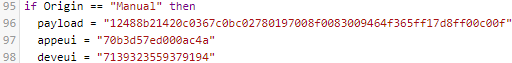
\includegraphics[width=0.9\textwidth]{images/8/manualInjection.png}
    \caption{Manual injection to test the smart script}
    \label{fig:manualInjection}
\end{figure}

\clearpage
\subsection{Code Size}
As well as the previous project, the results from the compilation in Mbed Studio is presented in the next figures. No changes to the default compilation profiles were done. 
\begin{figure}[H]
    \centering
    \begin{subfigure}[t]{0.45\textwidth}
        \centering
        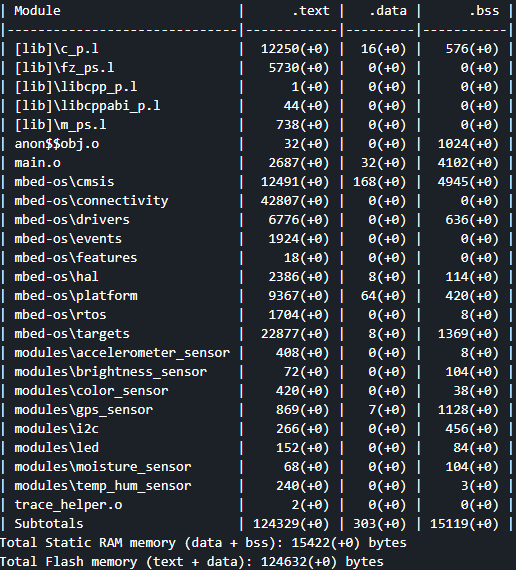
\includegraphics[width=0.882\textwidth]{images/8/debugSize.png}
        \caption{Debug compilation}
    \end{subfigure}
    \begin{subfigure}[t]{0.45\textwidth}
        \centering
        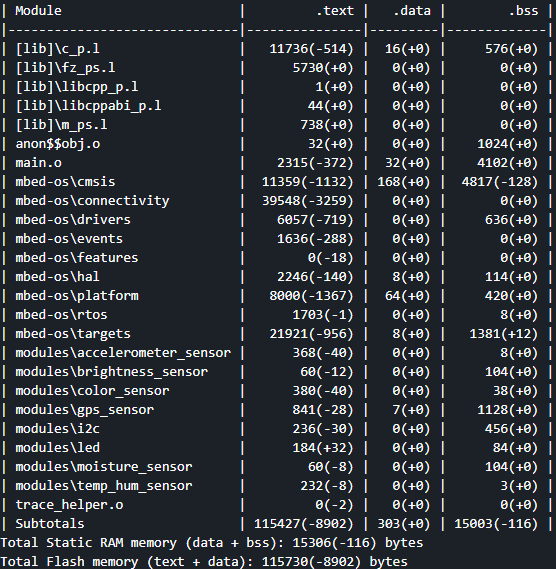
\includegraphics[width=0.95\textwidth]{images/8/developSize.png}
        \caption{Develop compilation}
    \end{subfigure}
    \begin{subfigure}[t]{0.45\textwidth}
        \centering
        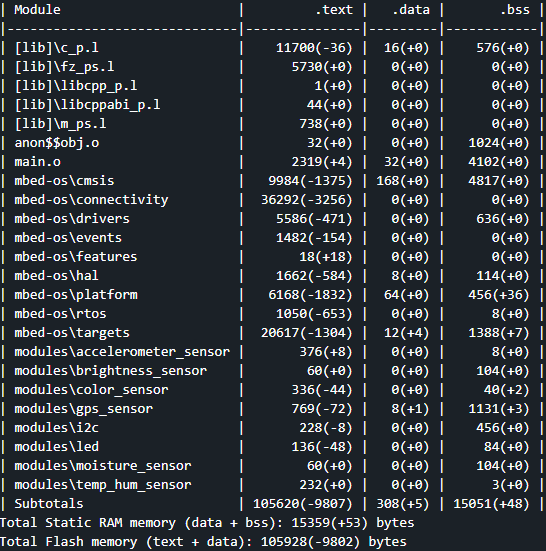
\includegraphics[width=0.95\textwidth]{images/8/releaseSize.png}
        \caption{Release compilation}
    \end{subfigure}
    \caption{Code size and module size for every compilation profile}
    \label{fig:compilation}
\end{figure}
\clearpage
